% Capítulo 4
\chapter{Fundamentação Teórica}\label{cap:fundamentacao-teorica}

Este capítulo está organizado para introduzir os conceitos-chave e explicar detalhadamente cada seção. Serão apresentados os fundamentos teóricos que sustentam o desenvolvimento e a aplicação de dois modelos fundamentais para a implementação da proposta: o modelo cognitivo e o modelo de template multicamadas para geração automática de questões. Cada subseção abordará os conceitos essenciais relacionados a esses modelos, detalhando suas características, funcionamento e contribuições para o objetivo final do estudo.

\section{Modelo Cognitivo}
A construção de questões em larga escala, por meio de processos automatizados, tem-se tornado uma prática cada vez mais relevante na área de avaliações educacionais. Nesse contexto, a elaboração de um modelo cognitivo sólido constitui um passo fundamental para embasar a Geração Automática de Questões (\gls{aig}). De modo geral, modelos cognitivos podem ser definidos como descrições explícitas de como os estudantes processam informações e resolvem tarefas específicas, envolvendo as habilidades e os raciocínios que se espera que demonstrem em uma dada questão. O processo de construção desse modelo, conforme discutido por \parencite{gierl2021}, esta técnica consiste em identificar, organizar e documentar de forma sistematizada os conceitos, parâmetros e restrições que caracterizam tanto a criação de uma questão quanto a forma como os estudantes são esperados a resolvê-la.

A relevância do modelo cognitivo torna-se ainda mais evidente quando se busca a replicabilidade e a qualidade das questões geradas em larga escala. Esse detalhamento fornece a base para a elaboração dos templates, os quais orientam a criação de questões capazes de manter o mesmo nível de complexidade, exigência cognitiva e alinhamento ao conteúdo que se deseja avaliar. Dessa forma, o modelo cognitivo funciona como um roteiro que descreve tanto os conteúdos quanto a lógica da questão a ser gerada.

O modelo cognitivo é a base fundamental para a criação dos templates, pois organiza e descreve todos os elementos necessários para sua construção. Os templates, por sua vez, atuam como estruturas que convertem essas informações de forma efetiva, resultando em questões de avaliação individual claras e alinhadas aos objetivos de ensino.


\section{Estrutura do Modelo Cognitivo}

O modelo cognitivo funciona como um guia para organizar os elementos necessários para a construção dos templates. Estes templates servem como estruturas que traduzem as diretrizes estabelecidas no modelo cognitivo em questões, claras, consistentes e alinhadas aos objetivos educacionais \parencite{keehner2017, gierl2017}. Para garantir a qualidade e replicabilidade, o modelo cognitivo deve ser estruturado de maneira a detalhar os seguintes aspectos fundamentais : 

\subsection{Problemas e Cenários}

A primeira etapa do processo de construção do modelo cognitivo consiste em definir claramente o objetivo da avaliação, identificando o problema central que servirá de base. Em uma disciplina de algoritmos que aborda estruturas de repetição, podemos optar por explorar aspectos como o tipo de laço ou os componentes fundamentais de uma estrutura controlada por um contador. Dessa forma, podemos assegurar que as habilidades específicas a serem avaliadas estejam claramente refletidas na questão. E, posteriormente, elaborar possíveis cenários relacionados ao problema principal. Nas avaliações sobre estruturas de repetição, podemos incluir cenários que envolvam a identificação do tipo de laço utilizado em um trecho de código, a utilização de contadores para controlar iterações ou a aplicação de estruturas de repetição em situações práticas de desenvolvimento de algoritmos. Cada cenário amplia a diversidade das questões, mantendo a coerência com o objetivo da avaliação.

\subsection{Fontes de Informação}

As fontes de informação constituem o conjunto de conteúdos e matérias que podem abranger dados quantitativos, textos, fórmulas, diagramas, trechos de código, figuras ou qualquer outro elemento que possibilite aos estudantes acionarem os conhecimentos e habilidades que se deseja avaliar. Cada fonte de informação deve ser descrita de forma detalhada, de modo a estabelecer claramente a relação entre o conteúdo apresentado e as características a serem avaliadas.


\subsection{Características (\textit{Features})}

As características (\textit{features}) são atributos fundamentais que compõem as dimensões ou variáveis do modelo cognitivo. Elas definem os aspectos que podem ser ajustados na criação dos templates. Na prática,cada característica é composta por três componentes principais: elementos, valores e restrições, descritos a seguir:

\begin{enumerate}
\item \textbf{Elementos} : Elementos representam as variações possíveis dentro de uma categoria ou dimensão específica da \textit{feature}, permitindo a manipulação do conteúdo através de componentes básicos que podem ser uma variável numérica, um trecho de código ou um termo técnico relevante para a questão. Os elementos devem ser construídos de forma a facilitar a combinação de um elemento com outro.

\item \textbf{Valores} : Valores são as possíveis combinações que os elementos podem assumir dentro de uma faixa de opções. Eles definem as variações quantitativas ou qualitativas que um elemento pode ter.

\item \textbf{Restrições} : Restrições são regras ou condições que limitam como os elementos e seus valores podem ser combinados. Elas garantem que as combinações resultantes sejam válidas, coerentes e alinhadas aos objetivos da questão, evitando a geração de questões inválidas ou sem sentido.

\end{enumerate}


A figura \ref{fig:cognitive-model} apresenta a estrutura hierárquica do modelo cognitivo para geração automática de questões, destacando os principais componentes e suas inter-relações. Ela organiza os elementos em três níveis principais : problemas e cenários, fontes de informação e características (\textit{features}). Essa visualização facilita o entendimento do processo de construção do modelo cognitivo.

\begin{figure}[ht]
	\centering
	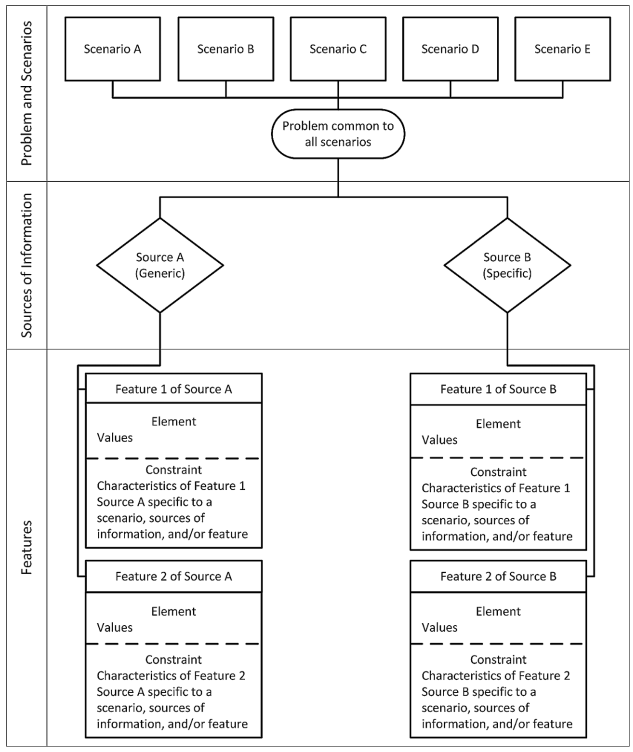
\includegraphics[width=12cm]{./imagens/capitulo4/cognitive-model}
	\caption{Estrutura do Modelo Cognitivo (Gierl, 2021)}
	\label{fig:cognitive-model}
\end{figure}


\section{Relação do Modelo Cognitivo e a Construção dos Templates }

O modelo cognitivo é o fundamento para a construção dos templates, pois organiza e descreve todos os conceitos, regras, parâmetros, limites e relações necessárias para a construção das questões. Os templates, por sua vez, convertem o modelo cognitivo em estruturas para gerar diferentes versões de questões, sendo assim a relação entre o modelo cognitivo e os templates pode ser resumida nos seguintes pontos:


\begin{enumerate} \item \textbf{Definição de elementos básicos de uma questão:} O modelo cognitivo descreve quais componentes  precisam estar presentes para que a questão seja relevante e alinhado aos objetivos de aprendizado. O \textit{template} organiza esses componentes em uma estrutura pronta para gerar diferentes versões de questão \parencite{lane2016}.

\item \textbf{Combinação e manipulação de parâmetros:}
Enquanto o modelo cognitivo define as regras de como os conteúdos e as habilidades podem ser combinados, o \textit{template} coloca essas regras em prática. Integra os diversos elementos para criar questões com diferentes níveis de complexidade, mantendo a coerência com a proposta original \parencite{embretson2017}.

\item \textbf{Padronização e escalabilidade:}
A adoção de um modelo cognitivo bem elaborado facilita a padronização do processo de elaboração de questões em grande escala. Como os \textit{templates} seguem o mesmo conjunto de regras e estruturas, as questões criadas tendem a manter consistência em termos de conteúdo, formato e nível de exigência cognitiva \parencite{gierl2017}.

\item \textbf{Validação e ajustes contínuos:}
Se um \textit{template} gerar uma questão que se revele incoerente ou sem lógica, é possível identificar rapidamente se o problema está no modelo cognitivo ou no próprio \textit{template}, permitindo o ajuste da regra que originou a inconsistência. Dessa forma, a correção ocorre em nível conceitual (no modelo) ou na estrutura do \textit{template}, preservando a qualidade das questões e mantendo-os alinhados aos propósitos da avaliação \parencite{gierlbulutzhang2018}.
\end{enumerate}


\section{Modelo Questão}

 Esta seção apresenta uma discussão sobre a construção de modelos de templates em diferentes níveis (\textit{1-layer, 2-layers, n-layers}) e a forma como esses modelos podem ser estruturados para permitir a geração de questões a partir de um único template, um modelo de questão pode ser descrito como um template que especifica os componentes manipuláveis de uma questão, e cada componente carrega um valor ou um intervalo de valores que podem ser alterados de forma sistemática para gerar novas questões \parencite{gierl2021}.

\subsection{Modelos de Template de uma camada (1-Layer)}

O modelo de item de 1-layer ("modelo de item de camada única") constitui uma abordagem na qual se manipulam apenas alguns elementos dentro de uma estrutura fixa para produzir novas questões. Este modelo é estruturado por um único template, onde cada elemento pode assumir diferentes valores previamente estabelecido \parencite{lai2013}. A seguir será apresentado as principais características desse modelo, sua forma de aplicações e limitações.

\subsection{Estrutura do Modelo}

O modelo de 1-layer parte de uma modelo cognitivo ou uma questão já existente com ponto de partida para identificar os elementos manipuláveis, e posteriormente isola-se os elementos variáveis da questão como números, termos, contextos que podem assumir diversas variações. Este modelo geralmente inclui : 

\begin{itemize}
    \item \textbf{Enunciado (Stem)} : Texto que apresenta a pergunta ou situação-problema
    \item \textbf{Elementos (Features)} : Constitui cada parte que pode mudar dentro do texto, todos os elementos estão em um só nível, compondo o corpo da questão. Esses elementos podem ser textos ou valores numéricos, em que cada elemento terá um intervalo ou conjunto de valores permitidos.
\end{itemize}

A Tabela \ref{tab:template-questoes-elementos} ilustra como a questão de referência se relaciona com o template e os respectivos elementos que podem variar. Na primeira linha, “\textbf{Questão de Referência}”, encontra-se o enunciado-base que exemplifica o problema a ser resolvido. Na segunda linha, “\textbf{Template (Stem)}”, temos a estrutura geral do enunciado, com espaços reservados para a inserção de diferentes conteúdos possíveis, podendo ainda incluir textos fixos que complementam o enunciado.

\begin{table}[htbp]
\centering
\begin{tabular}{|l|p{10cm}|}
\hline
\textbf{Questão de Referência} 
& Um e-commerce aplica descontos automáticos com base no valor do carrinho. Escreva um programa que receba o total da compra e, usando \texttt{if-else}, determine o desconto aplicado.  
\begin{itemize}
    \item Se o valor estiver entre R\$100,00 e R\$299,99, aplicar 5\%.
\end{itemize}
Após calcular o desconto, exiba o valor final da compra e a economia obtida. \\
\hline

\textbf{Template (Stem)} 
& \texttt{\{contexto-geral\} \{contexto-específico\} \{tabela-condicional\} \{solicitação\}} \\
\hline

\textbf{Elementos} 
& 
\begin{itemize}[leftmargin=1em]
  \item \textbf{contexto-geral}:
    \begin{itemize}[leftmargin=1em]
      \item Uma loja virtual está lançando promoções para fidelizar clientes em uma nova linha de produtos faciais.
      \item  Um supermercado online promove descontos para estimular compras em grandes quantidades durante as festas de fim de ano.
    \end{itemize}

  \item \textbf{contexto-específico}:
    \begin{itemize}[leftmargin=1em]
      \item A loja definiu descontos por faixa de valor no carrinho para aumentar as vendas.
      \item A loja oferece descontos progressivos em compras de livros nacionais conforme a condição a seguir:
    \end{itemize}

  \item \textbf{tabela-condicional}:
    \begin{itemize}[leftmargin=1em]
      \item Valor abaixo de R\$150,00: sem desconto.
      \item Entre R\$150,00 e R\$299,99: 5\%.
      \item Igual ou acima de R\$300,00: 10\%.
    \end{itemize}

  \item \textbf{solicitação}:
    \begin{itemize}[leftmargin=1em]
      \item Escreva um programa que calcule e aplique o desconto correto, exibindo o valor economizado.
      \item Crie um programa para calcular o valor final com base na faixa de desconto atingida.
    \end{itemize}
\end{itemize}\\
\hline

\end{tabular}
\caption{Template de Questões (Elaboração Própria, 2024)}
\label{tab:template-questoes-elementos}
\end{table}




\subsection{Processo de geração de questões com 1-Layer}

No modelo de uma camada (1-Layer), a geração de questões ocorre por meio da manipulação de um número limitado de elementos em um único nível do modelo. Essa abordagem é relativamente simples e de fácil implementação, pois se baseia em poucas variáveis para a criação das novas questões. Em razão dessa simplicidade, as variações ocorrem de forma linear, fazendo com que a diversidade das questões geradas seja menor. Ainda assim, este modelo é bastante útil quando se deseja alterar minimamente o contexto ou a a formulação geral, embora, por este mesmo motivo leva os estudantes a perceberem com mais facilidade padrões ou similaridades entre as questões geradas. 




\begin{table}[htbp]
\centering
\begin{tabular}{|l|p{10cm}|}
\hline
\textbf{Template (Stem)} 
& \texttt{[1]:\{contexto-geral\} [2]:\{contexto-específico\} [3]:\{tabela-condicional\} [4]:\{solicitação\}} \\
\hline
\textbf{Questão Gerada} 
& 
\begin{minipage}[t]{\linewidth}
\vspace{0.5em}
Uma loja virtual está lançando promoções para fidelizar clientes em uma nova linha de produtos.  
A loja oferece descontos progressivos em compras de livros nacionais conforme a condição a seguir:  
\begin{itemize}[leftmargin=1em]
    \item Se a compra for igual ou acima de R\$300,00, então o desconto será de 10\%.
\end{itemize}
Escreva um programa que calcule e aplique o desconto correto, exibindo o valor economizado. 
\vspace{0.5em}
\end{minipage} \\
\hline
\end{tabular}
\caption{Questão gerada (Autoria Própria, 2024)}
\label{tab:questao-gerada}
\end{table}



Como ilustra a Tabela \ref{tab:questao-gerada}, cada elemento variável é manipulado em um único nível, modificando-se apenas os índices dos itens pontuais tais como: contexto geral, contexto específico e solicitação para a geração de novas questões. Essa estrutura mais enxuta favorece a compreensão das etapas de modelagem, sendo indicada especialmente para professores que estão em fase de aprendizado na construção de \textit{templates}. Nesse sentido, o modelo \textit{1-layer} funciona como uma base inicial, antes de se evoluir para modelos mais complexos que exigem a manipulação de múltiplos níveis, como ocorre no modelo de \textit{n-layers}.

\subsection{Processo de geração de questões com  n-Layers}

A abordagem de multicamadas (\textit{n-layers}) amplia consideravelmente a capacidade de variação e a complexidade na geração de questões quando comparada ao modelo de camada única (\textit{1-layer}).  Enquanto que no modelo de uma camada é manipulado um pequeno conjunto de elementos em um \textit{template}, no modelo (\textit{n-layer}) cada camada adiciona uma nova estrutura de \textit{sub-templates} que possibilita combinar múltiplas estruturas de templates organizadas em níveis hierárquicos. Dessa forma, torna-se viável embutir os elementos, criando estruturas cada vez mais complexas que resultam em uma variedade maior  de questões geradas  \parencite{lai2013}. No entanto, essa maior diversidade traz também um aumento na complexidade de construção, pois a elaboração de modelos em múltiplas camadas requer planejamento adicional, tempo para projetar, validar e revisar cada camada e, sobretudo a experiência de quem elabora as questões \parencite{gierl2021}. 

Assim como no modelo de camada única, o ponto de partida do \textit{n-layer} é um um modelo cognitivo, que fornece os parâmetros principais de conteúdo, mas aqui cada layer pode conter blocos de informações e regras adicionais. À medida que se aumentam as camadas, introduzem-se mais cenários e variáveis e, portanto, aumentando a diversidade das questões geradas.


Considere a questão de referência ilustrada nas Figuras \ref{fig:questao-referencia-part-1} e \ref{fig:questao-referencia-part-2}. A primeira parte descreve um menu de calculadora; a segunda detalha três categorias de operação (fácil, moderado, e difícil), baseado neste modelo. Ao migrar para uma abordagem \textit{n‑layers}, é possível substituir o contexto de “calculadora” por múltiplos cenários similares a um menu, como por exemplo, interface de computador, caixa eletrônico, jogo simples, painel de controle industrial, sem alterar estrutura e a lógica de dificuldade da questão. Se, para cada nível de dificuldade, forem especificadas 20 variações e adotarmos apenas um cenário, já obtemos 20×20×20=8.000 variações. Com dois ou três cenários, esse quantitativo pode alcançar 16.000 ou 24.000 variações respectivamente, demonstrando o poder combinatório deste modelo.


\begin{figure}[ht]
	\centering
	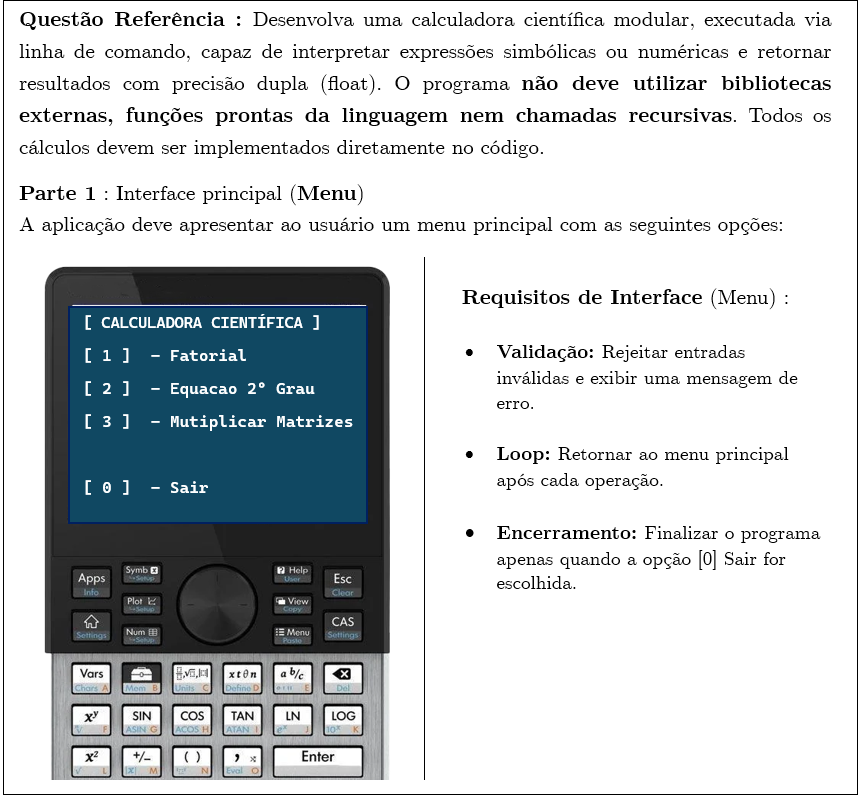
\includegraphics[width=12cm]{./imagens/capitulo4/questao-referencia-1.png}
	\caption{Questão de referencia - Parte 1 (Autoria Própria, 2025)}
	\label{fig:questao-referencia-part-2}
\end{figure}


\begin{figure}[ht]
    \centering
    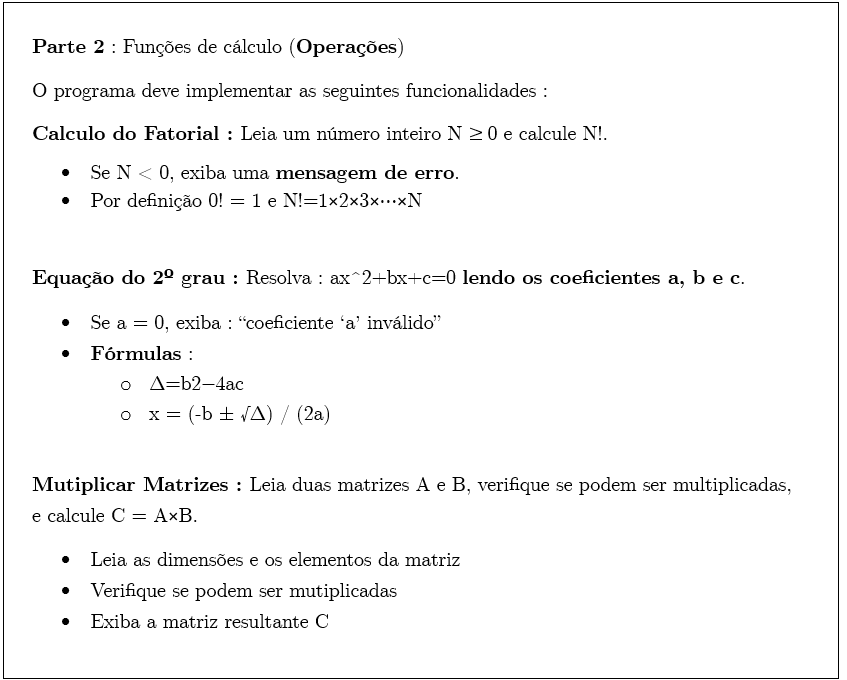
\includegraphics[width=12cm]{./imagens/capitulo4/questao-referencia-2.png}
    \caption{Questão de Referencia Parte 2 - Autoria Própria (2025)}
    \label{fig:questao-referencia-part-2}
\end{figure}

Em Paralelo com a geração automática de questões com aplicações em questões de medicina, no estudo de \parencite{gierl2021}, o template principal aborda doenças respiratórias, e as camadas seguintes eram detalhados cenários específicos para diagnosticar gripes (leve, moderada e severa) com bases nos sintomas apresentados. Aqui seguimos o mesmo raciocínio, o template principal fixa um contexto comum, e as subcamada especifica o contexto específico do contexto comum.

A Figura \ref{fig:template-1} e \ref{fig:template-2} mostra o modelo desta questão usando a abordagem multicamadas, onde o \textit{stem} (camada raiz) do template simula uma interface de uma calculadora, e os colchetes simples representam os pontos de variação, e os colchetes duplos subistituie a o subtemplate que será definido na camada seguinte, e cada indice numérico da lista é um valor possível que o template pode assumir. Isso permite reutilizar a estrutura original para substituir as variáveis sem comprometer a coerência da questão original.

\begin{figure}
    \centering
    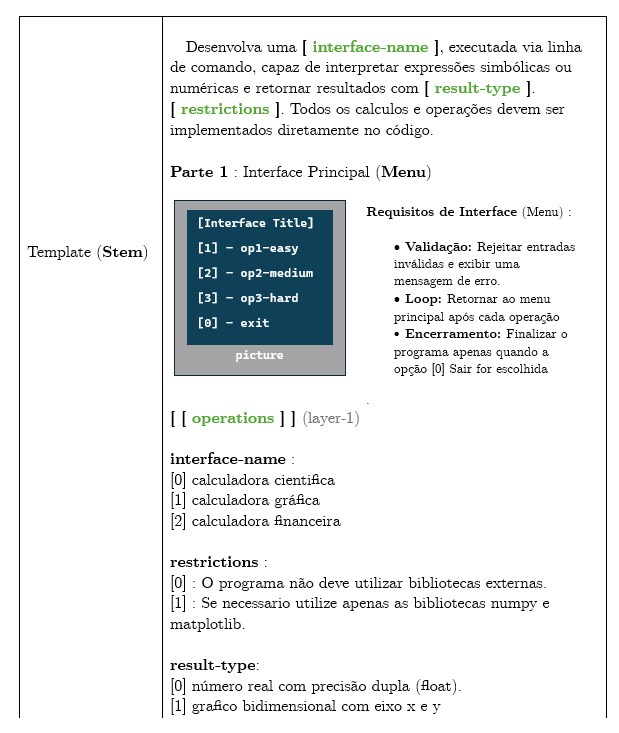
\includegraphics[width=12cm]{./imagens/capitulo4/template-1.png}
    \caption{Template Calculadora Parte 1 - Autoria Própria (2025)}
    \label{fig:template-1}
\end{figure}

\begin{figure}
    \centering
    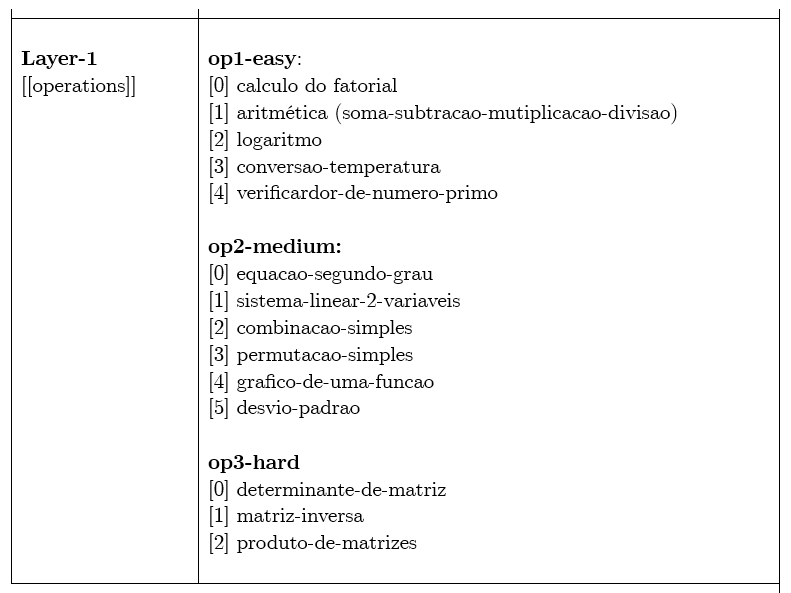
\includegraphics[width=12cm]{./imagens/capitulo4/template-2.png}
    \caption{Template Calculadora Parte 2 - Autoria Própria (2025)}
    \label{fig:template-2}
\end{figure}


\subsection{Razões para utilizar templates na geração de questões}

A geração automática de questões baseada em \textit{templates} é hoje uma estratégia versátil e operacionalmente viável para gerar questões em escala. A adoção de estruturas pré-definidas garante padronização, controle de complexidade e rastreamento dos erros, além de não exigir muitos recursos computacionais quando comparado com  as abordagens que não utilizam templates. Essas abordagens dependem de uma grande bases de dados e de modelos extensivamente treinados, que resulta em sua maioria, questões menos complexas, com criatividade limitada e com qualidade variável. Além disso, conforme \parencite{maity2024} menciona que, sistemas de geração automática de questões  baseadas em \gls{llm} tendem a gerar questões redundantes, enfrentam dificuldades na elaboração de problemas complexos, apresentam variação na qualidade das perguntas geradas e ainda estão sujeitos a riscos relacionados a vieses linguísticos. Estes fatores reforçam a atual preferencia pelo uso de \textit{templates} na geração automática de questões.